%================================================================
\chapter{Bayesian Inference}\label{chap:bayesian}
%================================================================

\epigraph{A decision was wise, even though it led to disastrous consequences, if the evidence at hand indicated it was the best one to make; and a decision was foolish, even though it led to the happiest possible con-\\sequences, if it was unreasonable to expect those consequences.}{Herodotus, around 500 BC}


The aim of statistical inference is to learn about underlying properties of a population from observed data.  In statistical inference, there are, broadly speaking, two paradigms for the analysis of observed data: \textit{frequentist} inference and \textit{Bayesian} inference. These often differ with each other on the fundamental interpretation of probability. In the frequentist view, the probabilities of events are defined as their relative frequencies in a repeatable objective process, and are thus ideally devoid of opinion. From a Bayesian perspective, probabilities are measures that quantifies the uncertainty level of statements based on the degree of belief about the state of the world. Probabilities can be assigned to any statement, even when a random process is not involved. Bayesian inference is the process of revising beliefs about the state of the world in the light of new evidence.     

This chapter introduces the fundamentals of Bayesian inference, with a particular focus on parameter inference. The content of this chapter is mainly based on the material in the Bayesian textbooks \cite{BDA}, \cite{BAP} and \cite{Sivia}.


%================================================================
\section{Bayes' Theorem}\label{sec:bayes_paradigm}
%================================================================

In terms of parameter inference, the Bayesian approach differs from the frequentist in that unknown parameters $\theta$ are treated as random variables rather than fixed quantities. In the Bayesian paradigm, all available information about an unknown parameter is incorporated in a \textit{prior probability distribution}, expressing our beliefs before some evidence is taken into account. We usually have a prior probability density function (pdf), $\prior$, since there will typically be a continuum of possible values of a parameter rather than just a discrete set. In the case of substantial prior knowledge about a parameter $\theta$, the prior pdf is narrow and concentrated about some central value, whereas a lack of information yield a wider and relatively flat prior pdf as shown in \autoref{fig:prior_illustration}. The prior is often specified by a particular distribution among a set of well-known and tractable distributions, with the purpose of making evaluation of prior probabilities and random generation of $\theta$ values straightforward.

\begin{figure}[H]
    \centering
    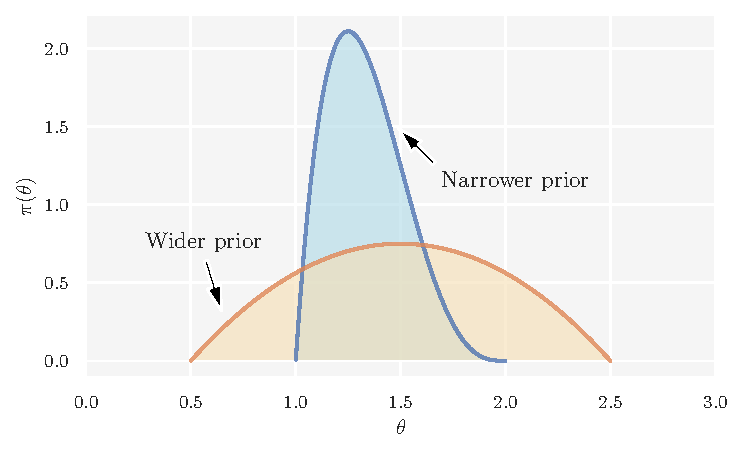
\includegraphics[scale=1.0]{prior_plot}
    \caption{Two prior distributions $\pi (\theta)$. A narrow concentrated prior (more certainty) about some central value and a wider less informative prior (less certainty).}
    \label{fig:prior_illustration}
    %\source{Figure 14.3 in \cite{STK}.}
\end{figure}

Our prior state of knowledge is modified by data $y$, obtained by performing experiments, through the conditional \textit{sampling distribution} $\lhood$. When regarded as a function of $\theta$, for fixed $y$, $\lhood$ is called the \textit{likelihood function}. In order to make probability statements about $\theta$ given sample data $y$, a probabilistic model representing the joint probability distribution for $\theta$ and $y$ must be provided. The joint pdf can be written as a product of the prior distribution $\prior$ and the likelihood function $\lhood$:

\begin{equation*}
    \joint = \lhood \prior .
\end{equation*}

At this point, Bayes' theorem is used to produce the \textit{posterior distribution}, which represents our state of knowledge about $\theta$ in the light of $y$. A common incarnation of Bayes' theorem is:

\begin{equation}\label{eq:bayes_theorem}
    \posterior = \frac{\joint}{p(y)}  = \frac{\lhood \prior}{p(y)},
\end{equation}

where the marginal probability of the data $p(y) = \int \lhood \prior \dd \theta$ in the case of continuous parameters, or, in the case of a discrete set of parameters, $p(y) = \sum_\theta \lhood \prior$, where the sum is over all possible values of $\theta$.

$p(y)$ is the same for all possible $\theta$, as it does not depend on $\theta$. With fixed $y$, this factor can thus be omitted in parameter inference since it constitutes a normalizing constant and does not enter into determining the relative posterior probabilities of different values of $\theta$. Omitting the factor $p(y)$ yields the unnormalized posterior distribution: 

\begin{equation}\label{eq:bayes_unnorm}
    \posterior \propto p(\theta, y) =  \lhood \prior .
\end{equation}

In this formulation, $\lhood$ is taken as a function of $\theta$ and not $y$.  

The core of Bayesian inference is encapsulated in \autoref{eq:bayes_theorem} and \autoref{eq:bayes_unnorm}. The principal task is to develop the joint probability model $\joint$ and perform the computations to obtain the posterior $\posterior$.


%================================================================
\section{Prior and Posterior Predictive Distributions}\label{sec:predictive_dist}
%================================================================  

Before observing any data $y$, we simply have the chosen model, i.e., the likelihood, $\lhood$, and the prior distribution of $\theta$, $\prior$. To make predictive inference about the expected future data, $\hat{y}$, encoded in the prior assumptions, we calculate the marginal distribution of $y$, that is, the distribution of $y \mid \theta$ averaged over all possible values of $\theta$:

\begin{equation}\label{eq:prior_pred}
    p \qty(\hat{y}) = \int \lhood \prior \dd{\theta}.
\end{equation}

\autoref{eq:prior_pred} is called the \textit{prior predictive distribution}. 

Once we have a posterior, it is possible to generate predictions $\hat{y}$ following a similar logic. The \textit{posterior predictive distribution} is calculated by marginalizing the distribution of $\hat{y} \mid \theta$ over the posterior distribution: 

\begin{equation}\label{eq:post_pred}
    p \qty( \hat{y} \mid y ) =\int p \qty(\hat{y} \mid \theta) \posterior \dd{\theta}.
\end{equation} 

Thus, the posterior predictive distribution is an average of conditional predictions over the posterior distribution of $\theta$.


%================================================================
\section{Parameter Inference}\label{sec:param_inference}
%================================================================  

The way in which Bayes' theorem operates is best seen through examples. In the following we discuss Bayesian inference in the context of a statistical model where the closed form is available. %Such models are sometimes unrealistic, but their analysis often provides a useful starting point when it comes to constructing more realistic models.  

%================================================================
\subsection{The Beta-Binomial Model and the Effect of Priors}\label{sec:coin_flipping}
%===============================================================

The beta-binomial model is one of the simplest Bayesian models, and useful for introducing important concepts and computational methods in Bayesian analysis. The model is often illustrated in the context of the classical coin-flipping problem, where only a single scalar parameter, the success probability $\theta$, is to be estimated. 

In the coin-flipping problem, we toss a coin $n$ times and record the observations: either \textit{heads} or \textit{tails}. Based on this data, we try to answer questions such as \textit{is the coin fair?} Or, more generally, \textit{how biased is the coin?} In order to estimate the bias of a coin in a Bayesian setting, we need observed data, a probabilistic model of the data generating process, i.e., the likelihood, and a prior placed on the unknown model parameter. For this example, we assume that the data-gathering part is already done and we have recorded the number of heads after a number of coin flips. The bias of the coin is represented by the $\theta$ parameter, and we say that a coin with $\theta=1$ will always land heads, one with $\theta=0$ always tails and one with $\theta=0.5$ has an equal chance of landing either heads or tails. Assuming that only two outcomes are possible, heads or tails, and the random variable \textit{coin toss} is independent and identically distributed (iid), a candidate for the likelihood is the binomial distribution: 

\begin{equation}\label{eq:coin_flip_likelihood}
    \lhood = \binom{n}{y} \theta^y \qty(1 - \theta)^{n-y}.
\end{equation}

This is a discrete distribution returning the probability of getting $y$ heads (or in general, successes) out of $n$ coin tosses (or in general, trials or experiments) given a fixed value of $\theta$ (probability of success). 

\autoref{fig:binom_distribution} illustrates the binomial distribution for different $\theta$. From the figure we see that $\theta$ indicates how likely it is to obtain a head when tossing a coin, making the binomial distribution a reasonable choice for the likelihood. 

\begin{figure}[ht]
    \centering
    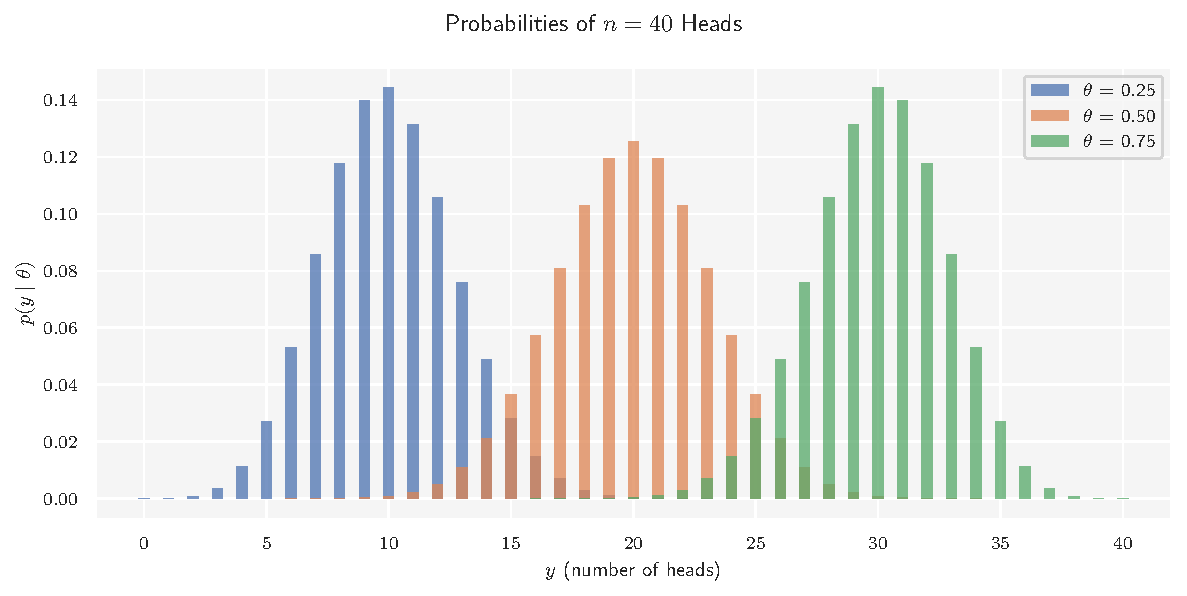
\includegraphics[scale=1]{binomial_distribution}
    \caption{Binomial distributions with $n=40$ coin flips and different success probabilities $\theta$. The coin is biased towards tails when $\theta < 0.5$ (blue) and heads when $\theta > 0.5$ (green). For $\theta=0.5$ (orange) the coin is unbiased (or fair). The legend indicates the values of the $\theta$.}
    \label{fig:binom_distribution}
\end{figure} 

If the value of $\theta$ is known, the binomial distribution tells us the expected distribution of heads. However, $\theta$ is an unknown model parameter, and thus we need to place a prior on it. For mathematical convenience, we choose a family of prior densities that lead to simple posterior densities. Considered as a function of $\theta$, \autoref{eq:coin_flip_likelihood} is of the form: 

\begin{equation*}
    \lhood \propto \theta^a \qty(1 - \theta)^b.
\end{equation*} 

If the prior density is of the same form, with its own parameterization of $a$ and $b$, then the posterior will also be of this form. Such a prior density can be parameterized as: 

\begin{equation*}
    \prior \propto \theta^{\alpha - 1} \qty(1 - \theta)^{\beta -1},
\end{equation*}

which is the beta distribution with shape parameters $\alpha>0$ and $\beta>0$. The parameters of the prior distribution are often called \textit{hyperparameters}. In order to ensure that the total probability is 1, the beta function,

\begin{equation*}
    B (\alpha, \beta) = \frac{\Gamma(\alpha)\Gamma(\beta)}{\Gamma(\alpha + \beta)},
\end{equation*}

where $\Gamma (z)$ is the gamma function, can be used as a normalizing constant:

\begin{equation}\label{eq:beta_prior}
    \prior = \frac{1}{B(\alpha, \beta)} \theta^{\alpha -1} (1-\theta)^{\beta -1}.
\end{equation}

The beta distribution is defined on the interval $[0, 1]$. \autoref{fig:beta_distribution} shows the beta distribution with different shape parameters. The figure displays the versatility of the beta distribution; the distribution adopts several shapes, determined by the shape parameters, including the uniform distribution with $\alpha = \beta = 1$. The uniform (blue) prior represents all the possible values for $\theta$ being equally likely a priori. The Gaussian-like (orange) prior is concentrated about $\theta=0.5$, and reflects a belief that the coin is equally probable to land heads or tails. The reverse J-shaped (green) prior is skewed towards a tail-biased outcome.

\begin{figure}[ht]
    \centering
    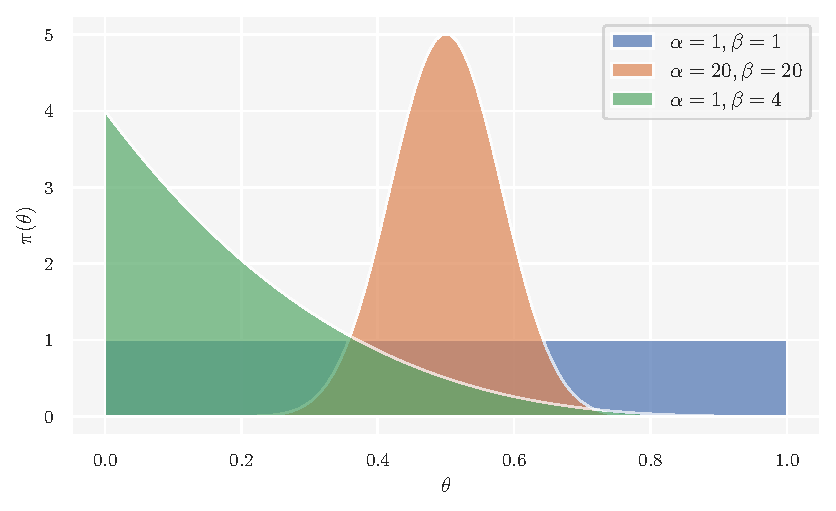
\includegraphics[scale=1]{beta_distribution}
    \caption{The beta prior probability distribution with different parameterizations by the two positive shape parameters. The beta distribution adopts several shapes controlled by the shape parameters; $\alpha=\beta=1$ gives a uniform distribution (blue), $\alpha=\beta=20$ gives a bell curve centered at $\theta=0.5$ (orange) and finally $\alpha=1$ and $\beta=2$ gives a reverse J-shaped distribution with a right tail (green).
    }
    \label{fig:beta_distribution}
\end{figure} 


Bayes' theorem, \autoref{eq:bayes_unnorm}, states that the posterior is proportional to the product of the likelihood and the prior. Thus, for our problem the posterior density for $\theta$ is given as: 

\begin{equation*}
    \pi (\theta \mid y) \propto \binom{n}{y} \theta^y (1-\theta)^{n-y} \frac{1}{B(\alpha, \beta)} \theta^{\alpha-1}(1-\theta)^{\beta -1}.
\end{equation*}

With fixed $n$ and $y$, the factor $\binom{n}{y}$ does not depend on the unknown parameter $\theta$, and neither does the beta function $B(\alpha, \beta)$. Thus can both be treated as constants when calculating the posterior distribution of $\theta$:

\begin{align*}
    \posterior &\propto \theta^y (1-\theta)^{n-y} \theta^{\alpha-1}(1-\theta)^{\beta -1} \\
    &= \theta^{\alpha + y -1} (1-\theta)^{\beta + n-y -1},
\end{align*}

or, more concisely:

\begin{equation}\label{eq:coin_posterior}
    \posterior \propto \theta^{\alpha' -1} (1-\theta)^{\beta' -1},
\end{equation}

with $\alpha'=\alpha+y$ and $\beta' = \beta + n - y$. We recognize that the expression above has the same functional form as the unnormalized beta distribution. The property that the posterior distribution follows the same parametric form as the prior distribution is called \textit{conjugacy}, and we say that the beta distribution is a \textit{conjugate prior} for the binomial likelihood.  

\autoref{fig:coin_flip_posterior} shows how the posteriors for the priors in \autoref{fig:beta_distribution} evolve as more and more data become available. For easier comparison, they have all been scaled vertically to have the same maximum value. \autoref{fig:coin_flip_posterior} clearly reveals the effect of the different priors; when there are few data, the shape of the posteriors vary in detail; as the number of data increases, the shape and location of the posteriors tend to converge and they all become sharply peaked. Since the priors reflect the different information or assumptions before the results, and the posteriors the updated knowledge in the light of data, this seems quite reasonable. If the data only are the outcome of a few flips, the analysis of these data is dominated by the prior information. However, as the data increases, the posterior is dominated by the likelihood and we are eventually led to the same conclusions regardless of our initial beliefs. In the limit of infinite data, all priors will provide the same posterior. From a practical point of view, we could obtain nearly indistinguishable posteriors for a finite amount of data. Thus, the choice of the prior becomes largely irrelevant given a sufficiently large amount of data.

\begin{figure}[!htb]
    \centering
    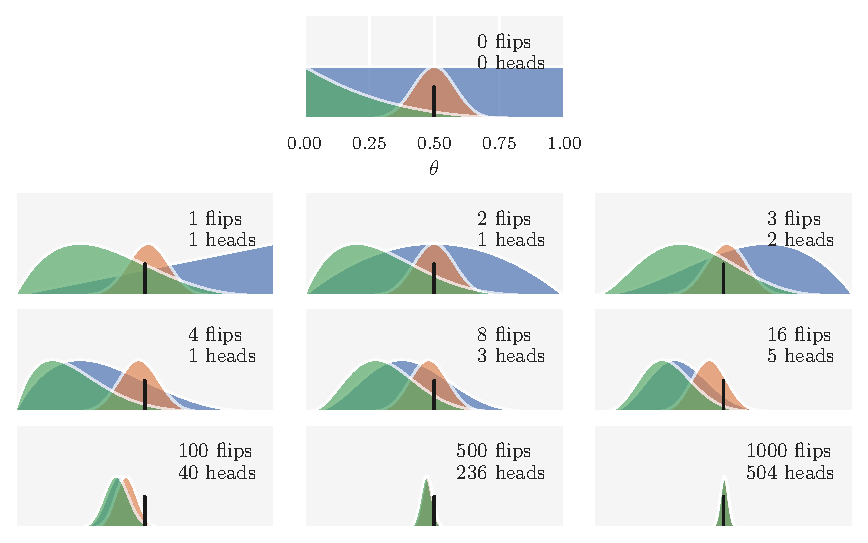
\includegraphics[scale=1]{coin_flip_posterior}
    \caption{The effect of different priors on the posterior as the number of data available increases. To aid in the comparison, they have all been scaled vertically to have the same maximum value. The number of data analyzed is indicated at the upper right-hand corner of each panel. In the first panel there are zero flips, and thus the densities represent the priors from \autoref{fig:beta_distribution}. The ground truth, $\theta=0.5$ (the coin is indeed fair), is indicated by the black vertical line. 
    }
    \label{fig:coin_flip_posterior}
\end{figure} 

Priors are often categorized by the information they incorporate about parameters as either \textit{noninformative}, \textit{weakly informative} or \textit{informative}. If the prior is noninformative, the posterior is data-driven, as illustrated by the uniform (blue) prior in \autoref{fig:coin_flip_posterior}. On the other hand, if the prior is informative, as illustrated by the bell curve (orange) prior in \autoref{fig:coin_flip_posterior}, the posterior is a mixture of the prior and the data. However, as mentioned and seen in the figure, the data will overwhelm the prior and dominate the posterior in the case of large amounts of data. Weakly informed priors are constructed to purposely include less information than we actually have. They can be useful if we want to let the data speak but not model complete ignorance.



%================================================================
\section{Bayesian Computation}\label{sec:bayesian_computation}
%================================================================

While conceptually simple, Bayesian analysis can be mathematically and numerically challenging. For a long time, Bayesians restricted their attention to conjugate families where posteriors can be computed analytically in closed form. However, realistic probabilistic models often lead to analytically intractable expressions. The arrival of the computational era and development of sampling-based numerical methods have transformed the Bayesian analysis practice. In this section we discuss estimating the posterior numerically using algorithms from the Markov Chain Monte Carlo (MCMC) family. 


%================================================================
\subsection{Markov Chain Monte Carlo}
%================================================================

There have been devised a suite of methods for constructing and sampling from arbitrary posterior distributions, but Markov chain Monte Carlo (MCMC) methods have become the predominant computational strategy for Bayesian inference. The term \textit{Monte Carlo} refers to methods that rely on the generation of random samples from a distribution of interest. In general, a \textit{Markov chain} is a sequence of states for which the probability of transitioning to the next state depends only on the present state. That the next state is only conditional on the present state and thus independent of the previous states is known as the Markov property. By providing a starting point, such a chain can perform a random walk between the states according to the transition probabilities. Hence, the main idea of MCMC is to draw samples of $\theta_t$ sequentially with the distribution of sampled draws depending on the previous sample $\theta_{t-1}$ to construct a Markov chain $\qty{\theta_t, t=0,1,2,...}$. The key to the method's success is finding a Markov chain with transitions proportional to the target posterior distribution, $\posterior$. In other words, the success is determined by whether the chain is able to improve the sampling distribution at each step in the simulations, in the sense of converging to the posterior distribution. 


%================================================================
\subsection{The Metropolis Algorithm}
%================================================================

The Metropolis algorithm is one of the most established MCMC sampling methods and was originally proposed in \cite{Metropolis}. It was later generalized by Hastings in \cite{Hastings} into the Metropolis-Hastings algorithm. In its original form, the Metropolis algorithm is an adaptation of a random walk that explores the local neighborhood of the current value of the Markov chain. It uses an acceptance/rejection rule to converge to the specified target distribution. The algorithm proceeds as follows:

\begin{enumerate}
    \item Initialize the Markov chain with a starting point $\theta_0$ for which $\pi \qty(\theta_0 \mid y)>0$. Conceptually, it makes most sense to draw $\theta_0$ from the prior $\pi(\theta)$, though it can be chosen by making an educated guess. 
    \item For each iteration of $t$, with $t=1, 2, ...$: 
    \begin{itemize}
        \item[(a)] Sample a \textit{proposal} parameter $\theta^*$ from the \textit{proposal distribution} (also called the \textit{jumping distribution}) $q \qty(\theta^* \mid \theta_{t-1})$ from which sampling is easily done. For the Metropolis algorithm (but not the Metropolis-Hastings algorithm), the proposal distribution must be symmetric, satisfying the condition $q \qty(\theta^* = \theta_a \mid \theta_{t-1} = \theta_b) = q \qty(\theta^* = \theta_b \mid \theta_{t-1} = \theta_a)$ for all $\theta_a$, $\theta_b$ and $t$. Both the normal and uniform distributions are examples of symmetric distributions that satisfies this condition. 
        \item[(b)] Evaluate the quality of the proposal $\theta^*$ by calculating the ratio of posterior densities: 
        \begin{equation}\label{eq:metropolis_ratio}
            r = \frac{\pi \qty(\theta^* \mid y)}{\pi \qty(\theta_{t-1} \mid y)} = \frac{p \qty(y \mid \theta^*) \pi \qty(\theta^*)}{p \qty(y \mid \theta_{t-1}) \pi \qty(\theta_{t-1})}.
        \end{equation} 
        Note that we do not actually use the posterior directly, but rather the proportionality given by Bayes' theorem (\autoref{eq:bayes_unnorm}). If the posterior density of $\theta^*$ is greater than that of $\theta_{t-1}$, the ratio of the posterior densities will be greater than 1 and we will accept the proposal as the next state of the chain. If the posterior density is greater for $\theta_{t-1}$, we will not necessarily discard the proposal $\theta^*$. Less probable parameter values are accepted probabilistically:
        \item[(c)] Calculate the Metropolis acceptance criterion:
        \begin{equation}\label{eq:metropolis_acceptance}
            \alpha = \min \qty(1, r),
        \end{equation}
        and set
        \begin{equation*}
            \theta_t = \begin{cases}
            \theta^* &\qquad \text{with probability } \alpha 
            \\
            \theta_{t-1} &\qquad \text{with probability } 1 - \alpha 
            \end{cases}.
        \end{equation*}
        In this way, the Metropolis algorithm ensures that the chain tends to move towards the highest density regions of the posterior, but it can still move away from these high-density regions and towards the tails of the posterior. The chain being able to assume all possible states, given enough time, is called \textit{ergodicity}, and is an important feature of the Metropolis algorithm. 
    \end{itemize}
\end{enumerate}

To implement the algorithm in a computer program, step (c) requires, after computing $\alpha$ for $\theta^*$, the generation of a uniform random number $u \sim \mathrm{U}(0,1)$. If $u \leq \alpha$, we accept the proposal and set $\theta_t = \theta^*$. If $u > \alpha$, we reject the proposal and set $\theta_t = \theta_{t-1}$ instead. Note that when the proposal is not accepted, this still counts as an iteration of the algorithm. 

The normal distribution, $\mathrm{N}\qty(\mu, \sigma^2)$, is an example of a symmetric proposal distribution. Conditioning the normal distribution on the previous value $\theta_{t-1}$ of the chain means that the location parameter $\mu=\theta_{t-1}$. The scale parameter $\sigma$ is a tuning parameter that we increase or decrease if the acceptance rate of the simulations is too high or low, respectively. According to \cite{BDA}, the optimal acceptance rate is 0.44 for single parameter inference problems and 0.23 for for inference problems concerning several parameters. 

\cref{alg:metropolis} summarizes the Metropolis algorithm.  

\begin{algorithm}[!htb]
\caption{Metropolis sampling}
\label{alg:metropolis}
\SetAlgoLined
\DontPrintSemicolon
 % Algorithm 
 \textbf{Inputs\,:}\;
 \vspace{-5mm}
 \begin{itemize}
     \item A target posterior density $\posterior \propto \lhood \prior$ consisting of a prior $\prior$ and likelihood $\lhood$. 
     \item A symmetric Markov proposal density $q \qty(\theta^* \mid \theta)$.
     \item An integer $N>0$.
 \end{itemize}
 
 \vspace{5mm}
 \textbf{Initialize\,:}\;
 \nl Sample $\theta_0 \sim \prior$.\;

 \vspace{5mm}
 \textbf{Sampling\,:}\;
 \For{$t=1, ..., N$}{ 
 \nl Generate proposal $\theta^* \sim q \qty(\theta^* \mid \theta_{t-1})$. \; 
 \nl Calculate acceptance criterion $\alpha = \min \qty(1, \dfrac{p \qty(y \mid \theta^*) \pi \qty(\theta^*)}{p \qty(y \mid \theta_{t-1}) \pi \qty(\theta_{t-1})})$. \;
 \nl Sample $u \sim \mathrm{U}(0,1)$. \; 
 \vspace{2mm}
 \eIf{$u \leq \alpha$}{
 \nl  $\theta_t = \theta^*$\;
   }{
  \nl $\theta_t = \theta_{t-1}$\;
  }
 }
\end{algorithm}



%================================================================
\section{Density Estimation}\label{sec:densest}
%================================================================ 

% \url{http://www.hep.caltech.edu/~fcp/statistics/densityEst/densityEst.pdf}

The probability density function (pdf) is a fundamental concept in statistics. When we estimate the posterior numerically, we obtain random samples of $\theta$ drawn from the posterior density $\posterior$ but not the posterior pdf itself. In this section, we briefly discuss \textit{density estimation}, that is, methods for constructing an estimate of the pdf from sample data. The focus will be on \textit{nonparametric} approaches to density estimation. It will be assumed that we are given a sample of $n$ univariate observations $x_1, ..., x_n$ whose underlying density is to be estimated. The density estimators will be denoted by $\hat{p}$. The content of this section is based on the material in the statistical learning textbooks \cite{ESL}, \cite{Bishop} and \cite{KDE_Porter}.

%================================================================
\subsection{Histograms} 
%================================================================

The most basic density estimator is the histogram. Standard histograms simply partition $x$ into $k$ bins of width $h$ and then count the number of observations of $x$ falling in each bin: 

\begin{equation*}
    h (x) = \sum_{i=1}^n B \qty(x - \tilde{x}_i ; h),
\end{equation*}

where $\tilde{x}_i$ is the center of the bin in which observation $x_i$ lies and 

\begin{equation*}
    B (x ; h) = \begin{cases}
    1 \qquad &\text{if } x \in \qty(-h/2, h/2) 
    \\
    0 \qquad &\text{otherwise}
    \end{cases}.
\end{equation*}

The histogram estimator for the pdf is then: 

\begin{equation}\label{eq:hist_densest}
    \hat{p}(x) = \frac{h(x)}{n h}
\end{equation}

This definition gives a density estimate $\hat{p}(x)$ that is constant over the width of each bin, and all bins have the same width $h$. The number of bins $k$ can be assigned directly or calculated from a suggested bin width $h$ as:

\begin{equation*}
    k = \left \lceil \frac{\mathrm{max}\, x - \mathrm{min}\, x}{h} \right \rceil, 
\end{equation*}

where the braces indicate the ceiling function. The amount of smoothing inherent in the procedure is primarily controlled by the bin width. Too small bin widths can give a density model with structure not present in the underlying data-generating density, and too large bin widths a density model that is too smooth for capturing the nuances of the underlying density. There are no hard-and-fast rules concerning the bin width, but there are some rules of thumb for setting $h$ based on $n$ and the dimensionality of the problem, such as Scott's rule \cite{scott_bin_width} and Freedman–Diaconis' rule \cite{freedman_diaconis}.

In practice, the histogram density estimator can be useful for quickly visualizing data in one or two dimensions, but is unsuited for most density estimation applications. For higher dimensional data, histograms are likely to run into the curse of dimensionality as the number of bins have an exponential scaling with the dimension. Another major issue is that the density has discontinuities that are due to the bin edges. \autoref{fig:kde_figure} in the next section provides an example of the histogram density estimator which illustrates this. However, the two important principles of density estimation are encapsulated in the histogram approach. First, in order to estimate the density at a particular location we should smooth the local neighborhood of that point. Second, the smoothing parameter should be neither too small nor too large to obtain an accurate estimate. The concept of locality requires some form of distance measure, and we have here assumed the Euclidean distance.

%================================================================
\subsection{Kernel Density Estimation}\label{sec:kde}
%================================================================

Kernel density estimates (KDEs) are closely related to histograms, but avoid some of the drawbacks. For instance, they have better scaling with dimensionality and can provide continuous density estimates. This is achieved by replacing the indicator function $B$ of the histogram density estimator with a standard \textit{smoothing kernel function}, defined by: 

\begin{equation}\label{eq:kernel_smooth_func}
    K_h \qty(\norm{x - x_i}) = \frac{1}{h} K \qty(\frac{\norm{x - x_i}}{h}),  
\end{equation}

where $h>0$ is the smoothing parameter, $\norm{\cdot}$ denotes the Euclidean distance  and $K(u)$ the kernel of a pdf. A kernel with subscript $h$ is usually referred to as a scaled kernel. The kernel estimator for the pdf is thus: 

\begin{equation}\label{eq:kde}
    \hat{p}(x) = \frac{1}{n} \sum_{i=1}^n K_h \qty(\norm{x - x_i}) = \frac{1}{nh} \sum_{i=1}^n K \qty(\frac{\norm{x - x_i}}{h}).
\end{equation}

The smoothing parameter $h$ is often called the \textit{bandwidth} in the context of kernel smoothing, and corresponds to the scale of the kernel. There are also rules-of-thumb for setting the bandwidth, such as Silverman's rule \cite{silverman_rule}. Intuitively, the kernel estimator is a sum of “bumps” placed at the sample points. The kernel determines the shape of the bumps and the bandwidth their width. \autoref{fig:kde_figure} provides an illustration of this, and also compares the histogram and kernel density estimate using the same data. The smoothness of the KDE compared to the discreteness of the histogram illustrates how KDEs converge faster to the underlying pdf.

\begin{figure}[!htb]
    \centering
    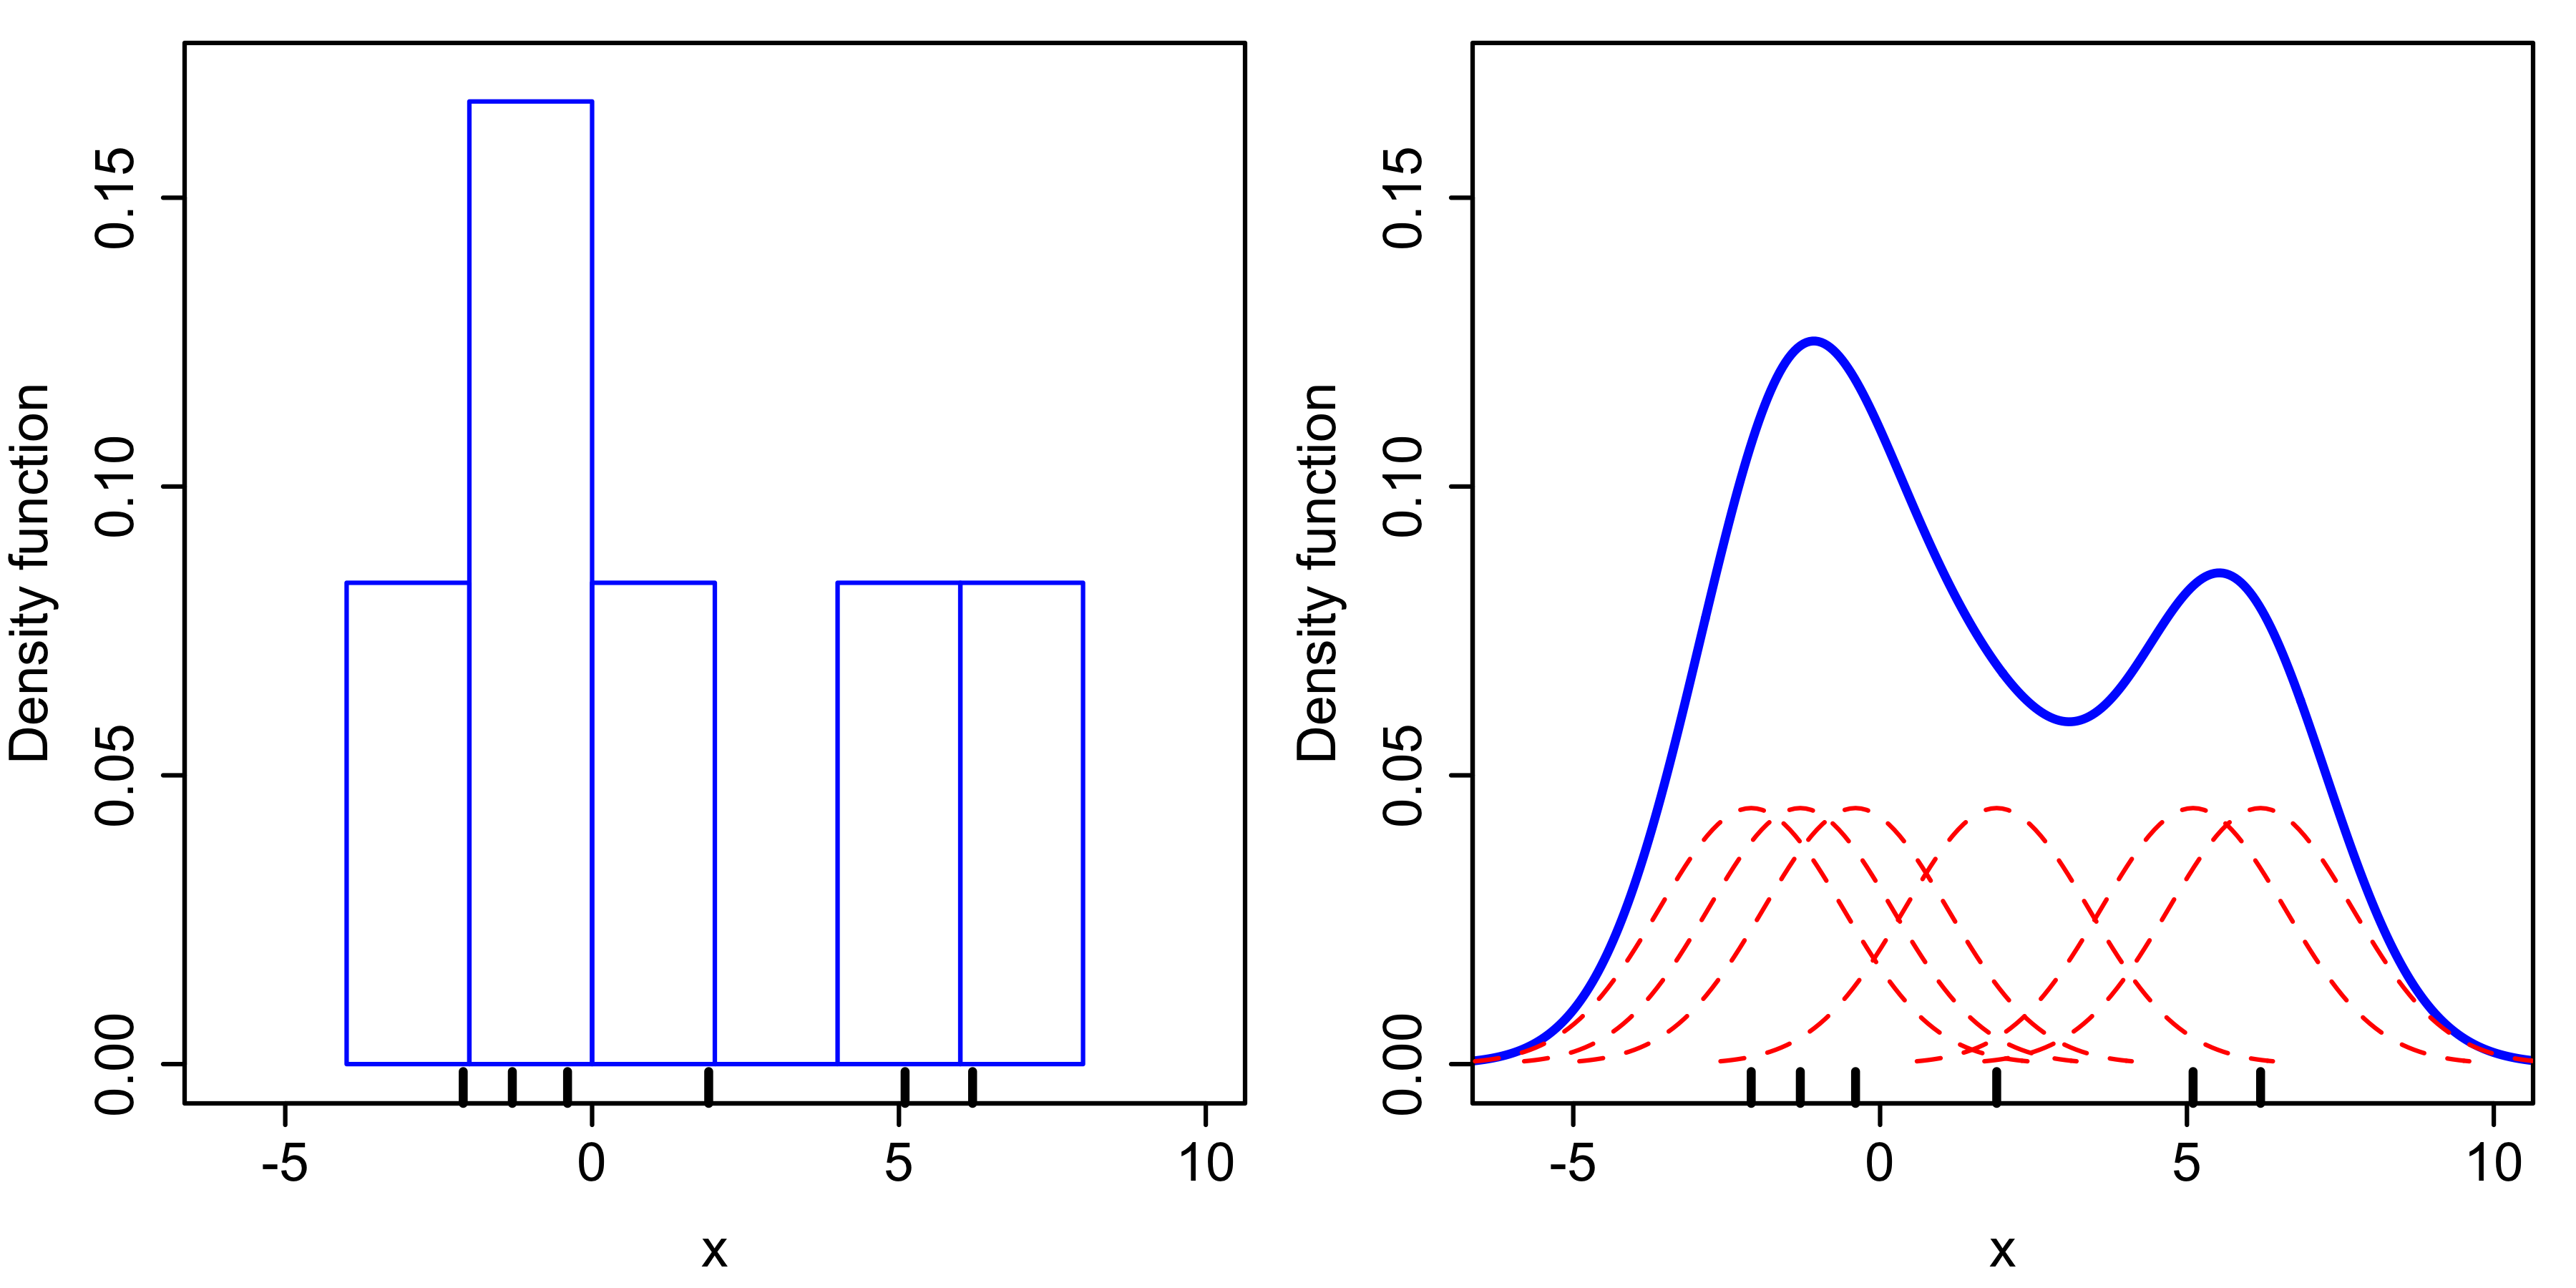
\includegraphics[scale=0.1]{Comparison_of_1D_histogram_and_KDE}
    \caption{Comparison of the histogram (left) and kernel density estimate (right) constructed using the same six data samples. For the histogram, the data is partitioned into $k=6$ bins, each of width $h=2$. If more than one data point falls inside the same bin, the density (height) of the bin increases. Note the discontinuities that are due to the bin edges. For the kernel density estimate (KDE), the kernel is Gaussian with bandwidth $h=2.25$. The kernel is placed on each of the six data samples (indicated by the red dashed curves), and the kernels are summed to make the KDE (solid blue curve). The data samples are shown as the rug plot on the horizontal axis.
    }
    \label{fig:kde_figure}
    \source{\cite{kde_figure}.}
\end{figure}


The kernel of a pdf is the form of the pdf in which any factors that are not functions of any of the variables in the domain are omitted. Kernels are symmetric functions such that $K(u) \geq 0$ for all $u$, $\int K(u) \dd{u}=1$ and $\int u^2 K(u) \dd{u} < \infty$. Some common choices of kernels are the Gaussian kernel:

\begin{equation}\label{eq:gaussian_kernel}
    K(u) \propto \exp(-\frac{1}{2} u^2),
\end{equation}

and the Epanechnikov kernel:

\begin{equation}\label{eq:epkov_kernel}
    K (u) \propto \begin{cases} 
    1 - u^2 \qquad &\text{if } \abs{u} \leq 1 
    \\
    0 \qquad &\text{otherwise}
    \end{cases}.
\end{equation}

\autoref{fig:kde_kernels} shows the Gaussian and Epanechnikov kernels. Kernels may or may not have finite support. Kernels with finite support are defined on a domain such as $[-1, 1]$, and kernels without on $(-\infty, \infty)$. The Gaussian kernel does not have finite support, while the Epanechnikov kernel has. 

\begin{figure}[!htb]
    \centering
    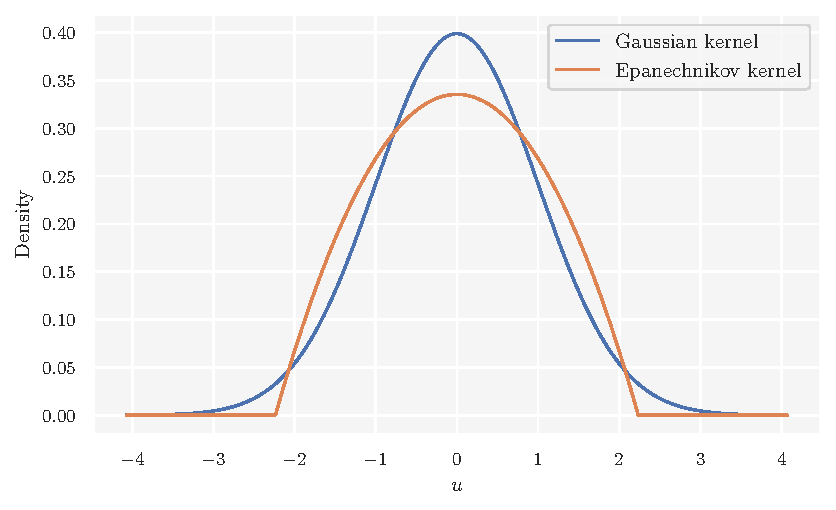
\includegraphics[scale=0.85]{kde_kernels}
    \caption{The Gaussian and Epanechnikov kernels defined by \autoref{eq:gaussian_kernel} and \autoref{eq:epkov_kernel}, respectively.
    }
    \label{fig:kde_kernels}
\end{figure}

%================================================================
\section{Summarizing the Posterior}
%================================================================ 

The result of a Bayesian analysis is a posterior distribution which contains all the current information about the parameters $\theta$. The focus of this section will be on how we can summarize the obtained posteriors.% with graphical checks and numerical measures.


\subsection{Visualization} 

Visualizing the posterior is a useful first-step in assessing the results of an inference, as the shape of the posterior quickly tells us how well the procedure was. However, we generally obtain estimated posterior samples and not the posterior density itself. In order to examine the location and width of the posterior, we therefore have to generate a visual representation by using density estimation, in particular KDE. If $\theta$ is a one- or two dimensional vector, we can simply plot the full posterior, which will be a joint posterior in the latter case. If the parameter vector has more than two dimensions, we can plot the marginal posterior for each parameter.

However, it is useful to also derive summary statistics from the posterior, as numerical summaries often are easier to present and interpret than the full posterior. 

\subsection{Bayesian Point Estimates}

\textit{Bayesian point estimates} are properties of the posterior. The most common point estimates, $\hat{\theta}$, are the:

\begin{itemize}
    \item Posterior mean: 
    \begin{equation}\label{eq:posterior_mean}
        \hat{\theta}_\mathrm{mean} = \E \qty[\theta \mid y] = \int \theta \posterior \dd{\theta}, 
    \end{equation}
    which simply is the expected value of the posterior distribution. 
    \item Posterior median: 
    \begin{equation}\label{eq:posterior_median}
        \hat{\theta}_\mathrm{median} = \mathrm{F}_{\theta \mid y}^{-1} \qty(0.5),
    \end{equation}
    where the cumulative posterior distribution $F_{\theta \mid y} \qty(\tilde{\theta}_q) = \int_{\infty}^{\tilde{\theta}_q} \posterior \dd{\theta}$. Here, $\tilde{\theta}_q$ is the value of $\theta$ at the $q$-quantile. For example, the median is the 0.5-quantile and the value of the cumulative posterior distribution is thus $F_{\theta \mid y} \qty(\tilde{\theta}_{0.5}) = 0.5$. The median being the $0.5$-quantile entails that it is the value of $\theta$ which divides the posterior in half.
    \item Posterior mode which is also called the maximum a posteriori probability (MAP) estimate: 
    \begin{equation}\label{eq:posterior_map}
        \hat{\theta}_\mathrm{MAP} = \max_\theta \posterior,
    \end{equation}
    and is the point at which the density is highest. 
\end{itemize}

As seen by the definitions above, each of the location summaries has its own interpretation. In general, there is no particular summary statistic that is preferred, and there will be different reasons to use each summary statistic. The mean is often used because it is a simple and familiar concept, or the observable is truly believed to be the average of some process. However, the mean might be a misleading point estimate for more complex and skewed distributions, such that $\hat{\theta}$ ends up in a region of low posterior density. The median is more robust to outliers than the mean, and we might prefer an estimate in the middle of the distribution. However, as with the mean, the median might also end up in regions of low density for more complex posteriors. The MAP estimate is closely related to the frequentist maximum likelihood estimate (MLE), and may be interpreted as the single “most likely” value. Providing an estimate of the MAP is more involved as we need to construct a KDE, which also may affect the quality of the estimate, based on the posterior samples and then find the mode of the KDE. The MAP estimate is most sensible to use for unimodal posteriors that have well-defined peaks. The MAP of a multimodal posterior might happen to be at one extreme and if the posterior is mostly flat the MAP might end up at an arbitrary location.  


\subsection{Posterior Uncertainty} 

In addition to posterior point estimates, it is important to report posterior uncertainty. The uncertainty can be characterized by the posterior standard deviation,

\begin{equation*}
    \mathrm{sd} \qty(\theta \mid y) = \sqrt{\mathrm{var}\qty(\theta \mid y)} = \sqrt{\int \qty(\theta - \bar{\theta})^2 \posterior \dd{\theta}},
\end{equation*} 

where $\mathrm{var}\qty(\theta \mid y)$ is the posterior variance and $\bar{\theta} = \E \qty[\theta \mid y]$ the posterior mean. The standard deviation works well for Gaussian-like distributions, but can be misleading for other, in particular skewed, distributions. An alternative is to use \textit{credible intervals} to quantify the posterior uncertainty. In the Bayesian paradigm, a credible interval is an interval within which $\theta$ falls with a particular probability. They are the Bayesian analogue of a frequentist confidence interval, though the interpretation, as usual, is different. In the Bayesian setting, an interval having a posterior probability $.95$ gives a 95\% probabilistic belief that the parameter is in that interval. A $100(1-\alpha)\%$ credible interval is a subset of $\theta$ such that

\begin{equation*}
    \int \posterior \dd{\theta} = 1 - \alpha,
\end{equation*}

where $\alpha$ is the confidence level. If the confidence level is $\alpha=0.05$, we have a 95\% credible interval. 

Credible intervals are not unique on a posterior. This means that we have to define a condition to construct a suitable interval. A common condition is to use the set of points for which the posterior density is higher than for any outside this set. This will be the narrowest interval on the posterior for some given confidence level, and is often referred to as the \textit{highest posterior density interval} (HPDI) or just the \textit{highest density interval} (HDI). 


\subsection{Posterior Predictive Checks}

The generated predictions $\hat{y}$ from the posterior predictive distribution, \autoref{eq:post_pred}, can be used to validate and criticize the model by comparing them with the observed data $y$. This is known as \textit{posterior predictive checks} (PPCs). The main idea of a PPC is to check for auto-consistency. The predicated data are simulated by typical posterior parameter values. If the predictions do not fit the observed patterns of interest, this might inform us on potential limitations of the model.  












